\chapter{Leader election evaluation}
\label{leaderelection}

\newcommand\algo[1]{\emph{#1} algorithm}
\newcommand\algocap[1]{\emph{#1} algorithm}
\newcommand\algoabbrv[1]{\emph{#1} algo.}

This chapter analyzes the performance of leader election in Raft, which
occurs when a leader fails and needs to be
replaced. Although we expect leader failures to be a rare event, they
should be handled in a timely manner. We would like Raft to reliably
elect a new leader in a fraction of a second in a typical deployment.

Unfortunately, it is difficult to put a bound on the time or number of
messages leader election will take. According to the FLP impossibility
result~\cite{Fischer:1985}, no
fault-tolerant consensus protocol can deterministically terminate in a
purely asynchronous model. This manifests itself in split votes in Raft,
which can potentially impede progress repeatedly during leader election.
Raft also makes use of
randomized timeouts during leader election, which makes its analysis
probabilistic. Thus, we can only say that leader election
performs well with high likelihood, and even then only under various
assumptions. For example, servers must choose timeouts from a random
distribution (they are not somehow synchronized), clocks must proceed at
about the same rates, and servers and networks must be timely (or
stopped). If these assumptions are not met for some period of time, the
cluster might not be able to elect a leader during that period
(though safety will always be maintained).

This chapter draws the following conclusions about the performance of
Raft's leader election algorithm:
%
\begin{itemize}
%
\item When no split vote occurs, elections complete about one third of
the way into the election timeout range, on average. They complete
slightly faster in clusters with more available servers, since the first
server is expected to time out sooner.
(Section~\ref{leaderelection:nosplit})
%
\item Split vote rates are low when the election timeout range is
sufficiently broad. We recommend a range that is
10--20 times the one-way
network latency, which keeps split votes rates under 40\% in all cases
for reasonably sized clusters, and typically results in much lower rates.
Clusters will experience more split votes as more servers fail, since
fewer votes are available. (Section~\ref{leaderelection:split:rate})
%
\item The number of election terms required to elect a leader follows a
geometric distribution,
where the expected number is $\dfrac{1}{1-\text{split vote rate}}$.
Thus, even a high split vote rate of 50\% will only need two election
terms on average to elect a leader.
A cluster configured with an election timeout that is 10--20 times its
one-way network latency will be able to elect a leader in less than 20
times its one-way network latency on average.
(Section~\ref{leaderelection:split:total})
%
\item Leader election performs well in practice in both local and wide
area networks. In a real-world LAN, our system was able to elect a
leader in an average of \SI{35}{\milli\second} when configured with aggressive
timeouts, though we suggest using a more conservative timeout range in
practice. On a simulated WAN spanning the US, elections typically
complete in half a second, and 99.9\% of elections complete in
\SI{3}{seconds}, even when two of five servers have failed.
(Section~\ref{leaderelection:lan})
%
\item The performance of leader election is not substantially affected
by the log comparison in RequestVote RPCs, when some servers will not
grant their votes to others. (Section~\ref{leaderelection:logsdiff})
%
\item The basic leader election algorithm can cause disruptions if
followers lose connectivity, increment their terms, and then regain
connectivity. Section~\ref{leaderelection:prevote} extends the basic
algorithm with an additional phase to avoid such disruptions.
%
\end{itemize}

\section{How fast will Raft elect a leader with no split votes?}
\label{leaderelection:nosplit}

\begin{figure}
\centering
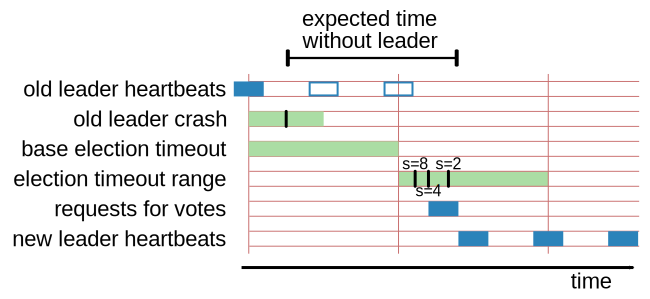
\includegraphics[scale=.55]{leaderelection/timeline}
\vcaption[leader election timeline with no split votes]{
Timeline of a typical election when no split vote occurs.
The first candidate to time out successfully collects votes and
completes the election (other elections may not be so fortunate). The
figure is drawn to scale assuming the election timeouts are chosen from
a range between 10--20 times the cluster's one-way network latency.
\\
The ``old leader heartbeats'' row shows the final heartbeat that the
old leader completes, and when it would have sent its next heartbeats
were it not to crash.
\\
The ``old leader crash'' row shows the interval during which the old
leader crashes. This time is assumed to follow a uniform random
distribution within its heartbeat interval. The vertical line halfway
through the interval is its expected (average) value.
\\
The ``base election timeout'' row shows the interval during which all
the followers await additional heartbeats from the old leader.
\\
The ``election timeout range'' row shows the interval during which the
servers would time out and start elections to replace the old leader.
The vertical lines show expected earliest timeout values for different
numbers of remaining servers (eight, four, and two, respectively).
\\
The ``requests for votes'' row shows when the candidate sends its
RequestVote RPCs to the other servers and receives their votes.
\\
The ``new leader heartbeats'' row shows the new leader sending out
heartbeat RPCs right away after becoming leader, then periodically
thereafter.
}
\label{fig:leaderelection:nosplit:timeline}
\end{figure}

The most common case for leader election in Raft is when no split vote
occurs, and this section analyzes how long it takes to elect a leader
under that assumption. This is expected to be the normal case for Raft
clusters; if the cluster is configured correctly, most normal elections
will not encounter a split vote. The first server to time out will be
able to collect votes from a majority of the cluster and become leader.
The timeline of events is shown in
Figure~\ref{fig:leaderelection:nosplit:timeline}. 

\begin{table}
\centering
\begin{tabular}{ccl}
variable & type & meaning \\
\hline
\noalign{\vskip .75ex}
$s$     & natural & number of available servers \\
$n$     & natural & size of full cluster (including unavailable servers) \\
$c$     & natural & number of servers to time out near each other \\
$l$     & time & constant half round trip network latency (special case of $L$)\\
$L$     & random variable of time & half round trip network latency \\
$W$     & random variable of time & time to write term and vote durably to disk \\
$T_i$   & random variable of time & timeout of server $i$ \\
$M_s$   & random variable of time & earliest timeout of $s$ servers \\
$D_{c,s}$ & random variable of time & difference in timeouts of earliest $c$ of $s$ servers \\
$E_s$   & random variable of time & time to complete an election \\
\end{tabular}
\vcaption[summary of variables]{
Summary of the variables used throughout this chapter to
analyze leader election performance.
Times are normalized to the election timeout range (ranging from 0 to
1).
}
\label{tab:leaderelection:variables}
\end{table}

\begin{figure}
\centering
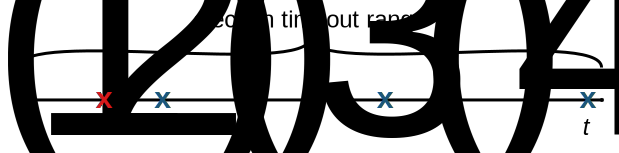
\includegraphics[scale=.5]{leaderelection/earliesttimeoutdiagram}
\vcaption[earliest timeout example]{
What is the smallest random election timeout value chosen by $s$
servers? The diagram shows random election timeouts a five-server
cluster where one server has failed ($s=4$). $t_{(1)}$ is the smallest
timeout value chosen.
}
\label{fig:leaderelection:theory:earliesttimeoutdiagram}
\end{figure}

With no split votes, the time it takes to elect a leader is determined
by how long it takes the first server to time out. The question of when
it will time out is illustrated in
Figure~\ref{fig:leaderelection:theory:earliesttimeoutdiagram}. Each server
waits for a uniform random timeout after the last time it received a
heartbeat. Intuitively, any individual server is expected to time out
halfway through the election timeout range, but with more servers it
becomes more likely that the first server will time out sooner.

We now define the problem more precisely and derive when the first
server times out analytically. The variables defined in this chapter are
summarized in Table~\ref{tab:leaderelection:variables}. Suppose each
server chooses its timeouts randomly from the standard
uniform distribution (in the range $[0,1]$). Let $T_1 \ldots T_s$ be
random variables representing when each of $s$ servers times out. Let $M_s$ be the minimum of
$T_1 \ldots T_s$, a random variable representing the time the first
server times out. Its cumulative distribution function (CDF) defines the
probability that $M_s$ is no greater than a particular time, $t$. This
is equivalent to one minus the probability that all servers times out
after $t$:
\begin{align*}
\Pr(M_s \leq t)
        &= 1 - \Pr(M_s > t) \\
        &= 1 - \prod_{i=1}^s \Pr(T_i > t) \\
        &= 1 - \prod_{i=1}^s (1 - t) \\
        &= 1 - (1-t)^s
\end{align*}
%
For example, consider a cluster with five servers where the prior
leader has failed.
The probability that the earliest of the remaining four servers times out
sometime in the first quarter of the election timeout range is
$\Pr(M_4 \leq \frac{1}{4}) = 1 - (1 - \frac{1}{4})^4 \approx 0.68$.
The CDF is graphed in
Figure~\ref{fig:leaderelection:theory:model:earliesttimeout}
for various values of $s$.

\begin{figure}
\centering
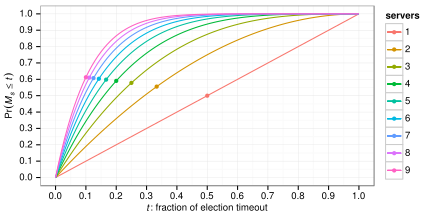
\includegraphics{leaderelection/earliesttimeout}
\vspace{-2ex}
\vcaption[earliest timeout CDF]{
The graph shows the probability that the earliest server times out
before $t$ when different numbers of servers are available. The point on
each line shows the time when the first server is expected to time out
($\Ex[M_s]$).
}
\label{fig:leaderelection:theory:model:earliesttimeout}
\end{figure}

The probability density function (PDF) of $M_s$ is the derivative of the
CDF:
\begin{align*}
 f_{M_s}(t) &= \frac{d}{dt} \Pr(M_s \leq t) \\
        &= \frac{d}{dt} (1-(1-t)^s) \\
        &= -\frac{d}{dt} (1-t)^s \\
        &= s (1-t)^{s-1}
\end{align*}

The expected value (mean) of $M_s$ is calculated from the PDF:
\begin{align*}
 \Ex[M_s] &= \int_0^1 \! t \, f_{M_s}(t) \, dt \\
          &= \int_0^1 \! t (s (1-t)^{s-1}) \, dt \\
          &= \left. \! -\frac{(1-t)^s (s\,t+1)}{s+1} \right|_{t=0}^1 \\
          &= \frac{1}{s+1}
\end{align*}

\noindent
For example, with four available servers, the first timeout is expected
to occur $\dfrac{1}{5}^\textrm{th}$ of the way through the election
timeout range. Fortunately, this very simple expression is a good
estimate of Raft's overall election performance, since elections
complete soon after the first candidate times out when no split vote
occurs.

More precisely, if there is no split vote, the full election requires
a candidate to time out and request votes, once the leader crashes:
\begin{align*}
E_s &= \text{baseline election timeout} + M_s + \text{time to request
votes} - \text{heartbeat adjustment} \\
E_s &= 1 + M_s + 2L + W - U(0,\dfrac{1}{2}) \\
\Ex[E_s] &= 1 + \frac{1}{s+1} + 2\Ex[L] + \Ex[W] - \dfrac{1}{4}
\end{align*}
where election timeouts are chosen from the range $[1,2]$,
$L$ is the network latency, and $W$ is the time to write the votes
persistently to disk.
A uniform random time value from the range $[0, \dfrac{1}{2}]$ is
subtracted, since leaders are expected to crash randomly within their
heartbeat intervals rather than immediately after sending heartbeats.

\section{How common are split votes?}
\label{leaderelection:split:rate}

The previous section analyzed the performance of normal elections when
no split vote occurs. In practice, two or more candidates may time out
at similar times, leading to split votes.  Split votes cause additional
election timeout delays, and if they occur too frequently, they can
impact election performance dramatically. This section first analyzes
split votes under a simplifying assumption that network latencies are
constant, then subsequently relaxes this assumption.

\subsubsection{Split vote rate with fixed latency}

\begin{figure}
\centering
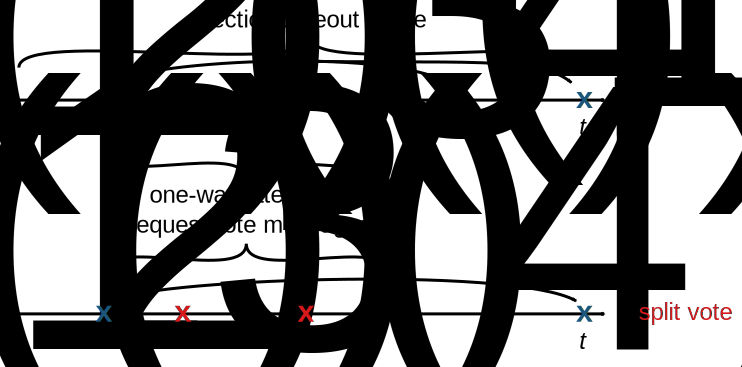
\includegraphics[scale=.5]{leaderelection/splitvotediagram}
\vcaption[split vote example with fixed latency]{
These examples show two similar elections in a five-server cluster when
one server has failed and network messages have a fixed latency. Each
server's random timeout value is shown on the timelines, where $t_{(1)}$
is the smallest value chosen, $t_{(2)}$ is the second-smallest, and so
on. In the top election, the first server is able to collect votes from
itself, the third server, and the fourth server. However, in the bottom
election, its RequestVote RPC cannot reach the third server in time
before that server times out; thus, the election ends in a split vote.
}
\label{fig:leaderelection:theory:splitvotediagram}
\end{figure}

Split votes can be calculated more simply if network latencies are
fixed. Let the constant $l$ be the one-way latency between any two
servers in the cluster, measured as a fraction of the election timeout
range.
Because of the fixed network latency,
the first server to time out is guaranteed to get the
votes of all servers that don't time out within $l$ of it, and it will
receive none of the votes of the other servers, who will each vote for
themselves.
The probability of a split vote is thus the probability that
too many candidates time out within $l$ of each other. For example,
consider a five-server cluster in which only four servers are available.
As illustrated in Figure~\ref{fig:leaderelection:theory:splitvotediagram},
if only two servers time out within $l$ of each other, the earliest server
will be able to collect votes from itself and the other two servers and
become leader. However, if three servers time out within $l$, then the
earliest server will only be able to reach one other server in time to
receive its vote, so the vote is split.

To derive a general formula for when split votes
occur, let $c$ denote the number of servers that time out within $l$ of
each other and let $n$ be the size of the full cluster.
The first server will get its own vote plus votes from the $s-c$ servers
that time out at least $l$ time after the first. Thus, a split vote
occurs when the following condition holds:
\begin{align*}
\text{votes needed}              &> \text{votes available to earliest server} \\
\Big\lfloor \dfrac{n}{2} \Big\rfloor + 1 &> 1 + (s - c) \\
c &> s - \Big\lfloor \frac{n}{2} \Big\rfloor
\end{align*}

How often split votes occur thus depends on how often at least $c$ servers
timeout within $l$ of each other. Let $D_{c,s} = T_{(c)} - T_{(1)}$,
where $T_{(i)}$ is a random variable representing the timeout of the
$i$-th of $s$ servers in sorted order; $D_{c,s}$ is the time after the
first server times out that the $c^\text{th}$ server times out. The
probability of split votes is then $\Pr(D_{c,s} < l)$, where $c$ is
determined by the formula given above ($s - \Big\lfloor \dfrac{n}{2}
\Big\rfloor + 1$).

We now derive the CDF for $D_{c,s}$, denoted $\Pr(D_{c,s} \leq l)$.
Suppose the first server times out at $t$.
%
First, if $t < 1-l$,
each of the following servers times out within $l$ time after $t$ with probability
$\dfrac{l}{1-t}$.
The probability that the second through $c^\text{th}$ servers time out
within $l$ time after $t$, and the remaining $s-c$ servers do not, is given by:
\begin{align*}
& \dbinom{s-1}{c-1}
  \left(\frac{l}{1-t}\right)^{c-1}
  \left(\frac{1-t-l}{1-t}\right)^{s-c}
\end{align*}
\noindent
%
Instead, if $t \geq 1-l$, then any server that times out after the first
must time out within $l$ time of $t$. Thus, all $s$ servers will
time out within $l$ of the first with probability $1$, and the
probability that any server does not timeout within $l$ of the first is
$0$. Putting this together, we can now derive the CDF:
%
\begin{align*}
\Pr(D_{c,s} \leq l)
%
 &= \mathlarger{\sum_{k=c}^s} \left(
\begin{aligned}
     &\int_0^{1-l}
     \Pr(\text{exactly $k$ servers time out in $t$ to $(t+l)$ range} \, | \, M_s=t)
     f_{M_s}(t) \, dt \, +
     \\
     &\int_{1-l}^1
     \Pr(\text{exactly $k$ servers time out in $t$ to $(t+l)$ range} \, | \, M_s=t)
     f_{M_s}(t) \, dt
\end{aligned}
\right) \displaybreak[0]\\
%
 &= \mathlarger{\sum_{k=c}^s}
     \left(
     \int_0^{1-l}
     \Pr(\text{exactly $k$ servers time out in $t$ to $(t+l)$ range} \, | \, M_s=t)
     f_{M_s}(t) \, dt
    \right) \, + \\
 &\quad \int_{1-l}^1 f_{M_s}(t) \, dt
  \displaybreak[0]\\
%
 &= \mathlarger{\sum_{k=c}^s}
     \left(
     \int_0^{1-l}
     \dbinom{s-1}{k-1}
     \left(\frac{l}{1-t}\right)^{k-1}
     \left(\frac{1-t-l}{1-t}\right)^{s-k}
     f_{M_s}(t) \, dt
    \right) \, + \\
 &\quad \int_{1-l}^1 f_{M_s}(t) \, dt
  \displaybreak[0]\\
%
 &= \mathlarger{\sum_{k=c}^s}
     \dbinom{s-1}{k-1}
     \left(
     \int_0^{1-l}
     \left(\frac{l}{1-t}\right)^{k-1}
     \left(\frac{1-t-l}{1-t}\right)^{s-k}
     s
     (1-t)^{s-1} \, dt
    \right) \, + \\
 &\quad \int_{1-l}^1 s (1-t)^{s-1} \, dt
  \displaybreak[0]\\
%
 &= \mathlarger{\sum_{k=c}^s}
     \dbinom{s-1}{k-1}
     \left. \left(
     -\frac{s}{s-k+1}
     l^{k-1}
     \left(1-t-l\right)^{s-k+1}
    \right) \right|_{t=0}^{1-l}
     \, + \\
 &\quad \mathlarger{\left. \left( -(1-t)^s \right)
\right|_{t=1-l}^1}
  \displaybreak[0]\\
%
 &= \left( \mathlarger{\sum_{k=c}^s}
     \dbinom{s-1}{k-1}
     \frac{s}{s-k+1}
     l^{k-1}
     (1-l)^{s-k+1}
    \right)
     \, + l^s
 \displaybreak[0] \\
%
 &= \left( \mathlarger{\sum_{k=c}^s}
     \frac{(s-1)! (s)}{(k-1)!(s-k)! (s-k+1)}
     l^{k-1}
     (1-l)^{s-k+1}
     \right)
     \, + l^s
    \displaybreak[0] \\
%
 &= \left(\mathlarger{\sum_{k=c}^s}
     \frac{s!}{(k-1)!(s-k+1)!}
     l^{k-1}
     (1-l)^{s-k+1}
     \right)
     \, + l^s
    \displaybreak[0] \\
%
 &= \left(\mathlarger{\sum_{k=c}^s}
     \dbinom{s}{k-1}
     l^{k-1}
     (1-l)^{s-k+1}
     \right)
     \, + l^s
    \displaybreak[0] \\
%
 &= \left(\mathlarger{\sum_{k=c-1}^{s-1}}
     \dbinom{s}{k}
     l^k
     (1-l)^{s-k}
     \right)
     \, + l^s
    \displaybreak[0] \\
%
 &= \mathlarger{\sum_{k=c-1}^s}
     \dbinom{s}{k}
     l^k
     (1-l)^{s-k}
    \displaybreak[0]
\end{align*}
%
(The CDF somewhat resembles a binomial distribution, which hints that
there may exist an easier derivation.)

For example, consider a five-server
cluster with four available servers ($s=4$). A split vote will occur if the
earliest three servers time out within $l$ of each other ($c=3$). If the
election timeout range is \SI{100}{\milli\second},
the earliest three servers will time
out within $l$ of each other, resulting in a split vote:
\begin{compactitem}
\item In about 0.06\% of elections, if the one-way network latency is
\SI{1}{\milli\second},
$\Pr(D_{3,4} \leq .01)$;
\item In about 5.2\% of elections, if the one-way network latency is
\SI{10}{\milli\second}, $\Pr(D_{3,4} \leq .1)$; and
\item In about 18.1\% of elections, if the one-way network latency is
\SI{20}{\milli\second}, $\Pr(D_{3,4} \leq .2)$.
\end{compactitem}

\begin{figure}
\centering
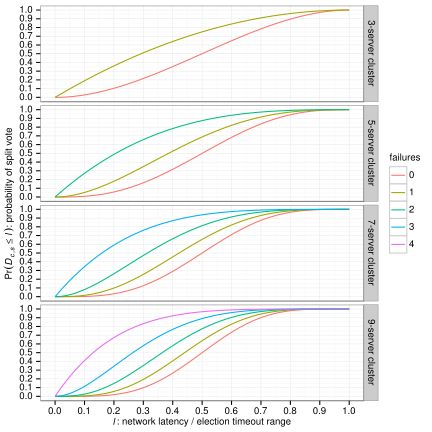
\includegraphics{leaderelection/distance}
\vspace{-2ex}
\vcaption[split vote probability with fixed network latency]{
The graphs show the likelihood of split votes for various cluster
sizes and numbers of server failures, given a fixed network latency $l$.
Each graph shows a different full cluster size, and the curves on each
graph show different numbers of failed servers in that cluster.
Each value represents the likelihood that a split vote will occur
because the first $c$ of the $s$ servers timed out within $l$ of each
other, where $c$ is determined by $s - \Big\lfloor \dfrac{n}{2}
\Big\rfloor + 1$.
For example, a five-server
cluster with two failures and $l=0.2$ will see about half of
elections end in split votes.
}
\label{fig:leaderelection:theory:distance}
\end{figure}


Figure~\ref{fig:leaderelection:theory:distance} graphs the CDF formula for
a range of cluster sizes. The first thing to observe is that failures
have a very large effect on split vote rates, especially if the cluster
is down to a bare majority of its original members. For example, a
five-server cluster
with $l=0.2$ will encounter less than 20\% split votes after one
failure;
if the same cluster encounters a second failure, about half of election
terms will encounter split votes. To prepare for worst-case scenarios,
the election timeout range should be set to produce tolerable values
when a bare majority of the cluster is available.

Second,
larger clusters experience fewer split votes with the same number of
failures, but they experience an even larger worst-case split vote rate
as a result of being able to tolerate more failures. For example, a
nine-server cluster with $l=0.2$ will experience only about a
15\% rate of
split votes after two failures (compare with 50\% for a five-server
cluster). However, when it is down to its bare majority with four
failures, the nine-server cluster will experience a nearly 70\% split vote rate.

Third, keeping the number of available servers constant, larger full
cluster sizes will have more split votes. For example, with $l=0.2$, a
nine-server cluster with six available servers will experience about a
35\% rate split votes; a seven-server cluster with six available servers will
experience only about a 10\% rate split votes. This is because larger full
clusters require more votes to win an election; fewer candidates need to
time out within $l$ of each other in order to produce a split vote.

Finally, the graphs suggest that choosing an election timeout range of
10--20 times the one-way network latency (so $l=0.1$) will result in low split
vote rates in all clusters, assuming network latencies are nearly
constant. With this setting, a nine-server cluster that has experienced
four failures will encounter 40\% split votes, and most typical clusters
will encounter much fewer. Smaller election timeouts (larger $l$ values)
may also work in many deployments, but they should be tested more
carefully to make sure.

\subsubsection{Split vote rate with variable latency}

When network latency is variable, calculating split vote rates is more
complicated. The problem is that a RequestVote message sent by one
server can overtake a RequestVote message sent earlier by a different
server. Thus, the first server to time out is no longer guaranteed to
collect all of the votes of servers that do not vote for themselves.
The first server is still the most likely candidate to win, by virtue of
sending requests for votes first, but its advantage depends on how much
earlier it timed out. Thus, with variable latency, we intuitively expect
somewhat higher rates of split votes (there is more competition).

\begin{figure}
\centering
\includegraphics{leaderelection/splits.pdf}
\vspace{-3ex}
\vcaption[split vote probability with variable network latency]{
The contour graphs show split vote rates for various cluster sizes and
numbers of failed servers. Each narrow contour line denotes a 1\%
increase in the probability of split votes; each medium contour line
denotes a 10\% increase; the thick contour line visible in some graphs
denotes the 50\% barrier. Split votes are always
0\% at the origin,
where messages are instantaneous. The points on the $x$ axis, where the
latency range is zero, correspond to the split vote rates with fixed
latencies in Figure~\ref{fig:leaderelection:theory:distance}.
\\
For example, the probability of a split vote for a five-server cluster
after one failure can be found in the graph in the second column and
second row. When latencies are chosen randomly and uniformly between 0.1
and 0.2, the point with a
minimum latency of 0.1 and a latency range of 0.1 reveals, by counting
contour lines, that the split vote rate is about 16\%. With two
failures, the probability of a split vote in the same cluster is nearly
40\%.
}
\label{fig:leaderelection:theory:splitvotes}
\end{figure}

Rather than model this mathematically, we used a small simulation. Each
run followed the following steps (before optimization):
%
\begin{enumerate}
%
\item Assign random timeouts to each of $s$ servers.
%
\item If a server has not voted by the time it times out, it votes for
itself and schedules RequestVote messages to be delivered to other
servers after random latencies.
%
\item If any server collects a majority of votes, the election term is
considered successful; otherwise, it is considered a split vote.
%
\end{enumerate}
%
After \num{10000} runs, the fraction of split votes was calculated.

Figure~\ref{fig:leaderelection:theory:splitvotes} shows the split vote
rates for messages with uniform random latencies in the range
$[l_\text{min},l_\text{max}]$, as calculated by the simulation.
(Uniform random latencies may not be a realistic distribution, but they
are the simplest case and can help with estimating more complex
distributions.)
The overall conclusion from these graphs is the same as
with fixed latency: more failures result in significantly higher split
vote rates.

In clusters with only a bare majority of servers available (the bottom
graph in each column), the contour lines are very linear with a slope of
about $-2$: they have about the same split vote rate when keeping the
average network latency constant. This indicates that the split vote
rates for bare-majority clusters
can be accurately approximated with our fixed latency model using
the average of the variable latency range. For example in a nine-server
cluster with four failures, a variable latency chosen randomly from the
range $[0.1, 0.2]$ results in a similar split vote rate as a fixed
latency of $0.15$.

In clusters with fewer failures, the contour lines aren't always linear,
and they typically have less slope in general (they are flatter). For
example, in a five-server cluster with no failures, a variable latency
between 0.1 and 0.2 has a similar split vote rate as a fixed latency of
about 0.2 (the slope of the contour lines is only about $-1$).
Typically, split vote rates can be bounded with our fixed latency model
using the maximum of the variable latency range. This is true for about
78\% of the data points shown in the figure; however, this approximation
works least well for large clusters with few failures, as these contour
lines are most curved.

\section{How fast will Raft elect a leader when split votes are possible?}
\label{leaderelection:split:total}

Given a split vote rate, we can estimate the total election time.
Raft will elect a leader as soon as an election term
successfully completes without a split vote. When a split vote occurs,
it's likely that all servers have reset their timers, since servers do
this when they grant a vote (this isn't quite true when logs
differ; see Section~\ref{leaderelection:logsdiff}). Thus, the
next election term has the same probability of success as an entirely
new election and will take just as long. In other words, each election
term is essentially memoryless, and the number of election terms
required in an election can be modeled as a geometric distribution,
where the probability of success is the probability that a split vote
does not occur. Therefore, Raft elections are expected to complete in
$\dfrac{1}{1-\text{split vote rate}}$ election terms on average.

If a split vote occurs in a particular election term, the election term
takes about $1+M_s$ time units plus a one-way network latency to reset
the server's election timers. We do not include the time for the
candidate to record its own vote on disk, since this time can be
overlapped with the RequestVote messages (with this optimization, the
candidate may not count its own vote towards leadership until the vote
is durably recorded). After the vote is split, the cluster must wait
another election timeout before the next election term begins. This
repeats for each split vote, then the time for an election with no split
votes (from Section~\ref{leaderelection:nosplit}) is additional. Thus, the
total time for an election, $E_s$, is:
\begin{align*}
E_s &= \Big(\sum_\text{split votes} \text{time for split vote}\Big)
 +
  \Big(\text{time for election with no split vote}\Big) \\
%
E_s &= \Big(\sum_\text{split votes} (1 + M_s + L)\Big)
 +
  \Big(1 + M_s + 2L + W - U(0,\dfrac{1}{2})\Big) & \\
%
\Ex[E_s] &= \Big((\frac{1}{1-\text{split vote rate}} - 1) \times
            (1 + \frac{1}{s+1} + \Ex[L])\Big)
 +
  \Big(1 + \frac{1}{s+1} + 2\Ex[L] + \Ex[W] - \dfrac{1}{4}\Big) \\
%
\Ex[E_s] &= \frac{1}{1-\text{split vote rate}} \times
            \Big(1 + \frac{1}{s+1} + \Ex[L]\Big)
            + \Ex[L] + \Ex[W] - \dfrac{1}{4}
\end{align*}
where $L$ is the one-way network latency and $W$ is the latency for a
durable disk write.

Howard~\cite{Howard:2014} suggests an optimization to decrease the time
for an election after split votes occur. The optimization separates
followers' timeouts from candidates' timeouts, where candidates select
smaller timeouts from a distribution with a smaller range. This results
in faster iterations once split votes have occurred, though it risks
additional split votes. The remainder of this chapter does not use this
optimization.

\begin{figure}
\centering
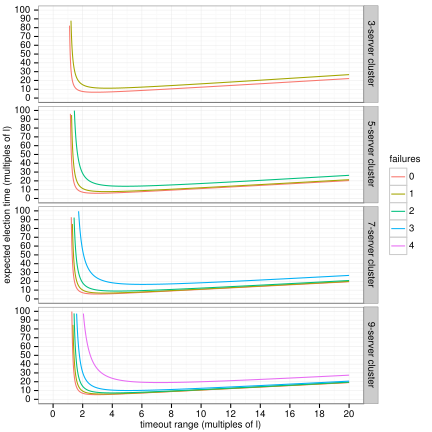
\includegraphics[height=5.5in]{leaderelection/overall}
\hspace{-2em}
\vcaption[expected overall election time]{
The expected total election times for various clusters,
as defined by $\Ex[E_s]$, with a fixed one-way network latency.
It excludes the time to write to stable
storage (which is usually negligible). The timeout range and
expected overall election time are presented as multiples of the one-way
network latency ($l$), since $l$ is typically fixed in a given
deployment.
}
\label{fig:leaderelection:theory:overall}
\end{figure}

Figure~\ref{fig:leaderelection:theory:overall} plots the expected time to
elect a leader when the network latency is fixed, by combining the
formula for $\Ex[E_s]$ with the formula for $Pr(D_{c,s} \leq l)$.
From the graphs, a Raft cluster with a sufficiently broad timeout range
will usually elect a leader within 20 times the one-way network latency,
even when running with a bare majority of available servers. This
suggests that most datacenter Raft deployments should be able to achieve
typical leader election times under \SI{100}{\milli\second}. Even worst
case global deployments, with one-way latencies of
\SI{200}{\milli\second},
should be able to typically elect leaders within \SI{4}{seconds}. (Election
times may be larger if some servers are deployed on other planets.)

Each of the curves has a knee. If the timeout range is chosen to be too
short, too many servers time out before others are able to collect
votes, resulting in poor election times. Once timeout ranges are
sufficiently large (about 3--8 times the network latency, depending on
the cluster), the curves become linear with a slight upward slope:
elections complete after few or no split votes, but they must wait
longer for each timeout to elapse.

The graphs provide insight into how to configure election timeouts: a
conservative setting is probably best in practice. The minimum point on
the graphs represents the best average election time possible for each
given cluster configuration. However, attaining this minimum time is
quite risky, since the minimum is close to the knee in the curve. If the
network latency turns out to be slightly higher than anticipated in
practice, that might push the system into the left region of the graph
where election times skyrocket. It is better to configure systems
farther to the right, trading off a slightly higher average election
time in exchange for a more robust system. Thus, we recommend using a
timeout range that is ten times the one-way network latency (even if the
true network latency is five times greater than anticipated, most clusters would
still be able to elect a leader in a timely manner).

\section{How fast will the complete Raft algorithm elect a leader in
real networks?}
\label{leaderelection:lan}


The previous sections were based on simplified models of how leader
election works in Raft. We wanted to know how fast Raft will be able to
elect a leader in the real world. To find out, this section evaluates
Raft's leader election algorithm using a real-world benchmark in a LAN
environment and a realistic simulator in a slower WAN environment.

\subsubsection{Real-world implementation on a LAN}

\begin{table}
\centering
\begin{tabular}{r l}
code & LogCabin~\cite{logcabin}, written in C++11 \\
OS & x86-64 RHEL6 (Linux 2.6.32) \\
CPU & Xeon X3470 (4 cores, 8 hyperthreads) \\
disk & ext4 file system on Crucial M4 SSDs (1 SSD per server) \\
network & Protocol Buffers~\cite{Varda:2008} over TCP/IP over 1~gigabit Ethernet \\
configuration & in-memory state machine, no log compaction \\
\end{tabular}
\vcaption[experimental setup for benchmark]{
Experimental setup for real-world LAN benchmark.
}
\label{tab:leaderelection:benchmarksetup}
\end{table}

We used LogCabin to measure the performance of Raft's
leader election algorithm on five servers connected by a gigabit Ethernet network.
The experimental setup is summarized in
Table~\ref{tab:leaderelection:benchmarksetup}. The benchmark repeatedly
crashed the leader of a cluster of five servers and timed how long it
took to detect the crash and elect a new leader. The benchmark measured
the time from when the old leader crashed until the other servers
received the new leader's first heartbeat (see
Figure~\ref{fig:leaderelection:nosplit:timeline}). The leader was crashed
randomly within its heartbeat interval, which was half of the
minimum election timeout for all tests. Thus, the smallest possible
downtime was about half of the minimum election timeout.

\begin{figure}
\centering

\begin{subfigure}{\textwidth}
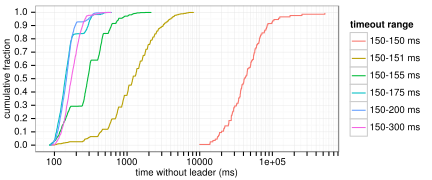
\includegraphics{leaderelection/benchmarks-randomness}
\caption{
Time to elect new leader when varying the range of randomness in
election timeouts.
}
\label{fig:leaderelection:benchmark-randomness}
\end{subfigure}

\vspace{4ex}

\begin{subfigure}{\textwidth}
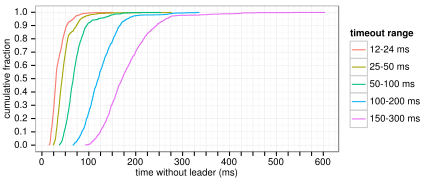
\includegraphics{leaderelection/benchmarks-scale}
\caption{
Time to elect new leader when scaling the minimum election timeout.
}
\label{fig:leaderelection:benchmark-scale}
\end{subfigure}

\vcaption[benchmark results on LAN cluster]{
The graphs show the time to detect and replace a crashed leader in the
real-world LAN benchmark. Each line represents \num{1000}
trials (except for 100 trials for ``\SIrange{150}{150}{\milli\second}'')
and corresponds to a
particular choice of election timeouts; for example,
``\SIrange{150}{155}{\milli\second}''
means that election timeouts were chosen randomly and uniformly between
\SI{150}{\milli\second} and \SI{155}{\milli\second}.
The steps that appear on the graphs show when split votes occur (the
cluster must wait for another election timeout before a leader can be
elected).
The measurements were taken on a cluster of five servers with a
broadcast time (network round trip plus disk write) of roughly
\SI{15}{\milli\second}.
Results for a cluster of nine servers are similar.
}
\label{fig:leaderelection:benchmark}
\end{figure}

The benchmark tried to generate a worst-case scenario for leader
election. First, it synchronized the old leader's heartbeat RPCs before
causing the old leader to exit; this made the follower's election timers
start at approximately the same time, leading to many split votes if the
timeout values were not sufficiently randomized. Second, the servers in
each trial had different log lengths, so two of the four servers were not
eligible to become leader (however, Section~\ref{leaderelection:logsdiff}
will show that this has only a minor effect on election times).

Figure~\ref{fig:leaderelection:benchmark-randomness} shows that elections
complete in under one second when the timeout range is sufficiently
broad. A small amount of randomization in the election timeout is enough
to avoid split votes in elections. In the absence of randomness, leader
election consistently took longer than \SI{10}{seconds} due to many split
votes. Adding just \SI{5}{\milli\second} of randomness helps
significantly, resulting in
a median downtime of \SI{287}{\milli\second}.
Using more randomness improves worst-case
behavior: with a \SI{50}{\milli\second} random range, the worst-case
completion time
(over \num{1000} trials) was \SI{513}{\milli\second}.

Figure~\ref{fig:leaderelection:benchmark-scale} shows that downtime can
be reduced by reducing the election timeout.
With an election timeout of
\SIrange{12}{24}{\milli\second}, it takes only
\SI{35}{\milli\second} on average to elect a leader
(the longest trial took \SI{152}{\milli\second}).
However, lowering the timeouts beyond this point violates Raft's timing
requirement: leaders have difficulty broadcasting heartbeats before
other servers start new elections. This can cause unnecessary leader
changes and lower overall system availability.
We recommend using a conservative election timeout such as
\SIrange{150}{300}{\milli\second};
such timeouts are unlikely to cause unnecessary leader changes, result
in a low rate of split votes, and will still provide good availability.

\subsubsection{Simulated WAN network}

We developed a simulator called AvailSim~\cite{availsim} to
explore a wider range of leader election scenarios. Unlike the
fixed network in our real-world test cluster, AvailSim allows the
latency of the simulated network to be configured arbitrarily.
(We used AvailSim to interactively explore a wide space of leader
election scenarios and algorithms, but this chapter only includes a few
relevant results.)

AvailSim is a close approximation to a complete Raft system, but its
election time results differ from real elections in two ways:
%
\begin{enumerate}
%
\item Each server in AvailSim begins with a fresh election timer. In
practice, the leader will crash at some random point in time between
heartbeats. The election times produced by AvailSim are thus an average
of half a heartbeat interval too large.
%
\item AvailSim does not add any time for processing messages or writing
to disk (these are infinitely fast in the simulator). CPU time should be
short relative to network latency, and disks need not play a significant
role in leader election anyhow (see
Section~\ref{leaderelection:split:total}).
%
\end{enumerate}

\begin{figure}[p]
\centering
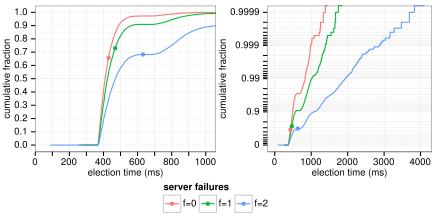
\includegraphics{leaderelection/multi-submission-failures}
\vspace{-4ex}
\vcaption[election performance on a simulated WAN cluster]{
Election performance as calculated by AvailSim for a WAN (one-way
network latency of 
\SIrange{30}{40}{\milli\second}). The figure shows a cluster of
five servers with zero, one, and two servers having failed.
\\
The left graph plots the CDFs of election times. The right graph plots
the same curves on a reverse-logarithmic $y$ axis to magnify
detail on the tail of the distribution. Each CDF summarizes \num{10000}
simulated elections. The point on each curve marks the average election
time.
}
\label{fig:leaderelection:simulation:dist:submission-failures}
\end{figure}

\begin{figure}[p]
\centering
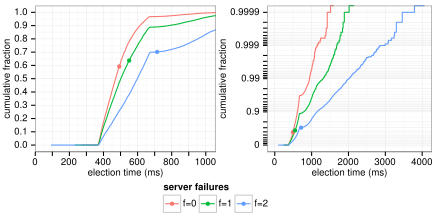
\includegraphics{leaderelection/multi-submission-failures-logsdiff}
\vspace{-4ex}
\vcaption[election performance with differing logs]{
Election performance as calculated by AvailSim when each server has a
different log (using the same WAN configuration as
Figure~\ref{fig:leaderelection:simulation:dist:submission-failures}).
Performance is similar to
Figure~\ref{fig:leaderelection:simulation:dist:submission-failures}, where
the servers' logs are all the same.
}
\label{fig:leaderelection:simulation:dist:submission-failures-logsdiff}
\end{figure}

We used AvailSim to approximate a WAN spanning the continental US. Each
message was assigned a latency chosen randomly from the uniform range of
\SIrange{30}{40}{\milli\second}, and the servers' election timeout range was set
accordingly to \SIrange{300}{600}{\milli\second} (about 10--20 times the
one-way network latency).

Figure~\ref{fig:leaderelection:simulation:dist:submission-failures} shows
how quickly a five-server cluster elects a leader in this WAN
environment. When only one of the five servers has failed, the average
election completes within about
\SI{475}{\milli\second}, and 99.9\% of
elections complete within
\SI{1.5}{\second}. Even when two of the five servers
have failed, the average election takes about
\SI{650}{\milli\second} (about 20
times the one-way network latency), and 99.9\%
of elections complete in
\SI{3}{\second}. We believe these election times are more than adequate for
most WAN deployments.

\section{What happens when logs differ?}
\label{leaderelection:logsdiff}

Most of this chapter has assumed that servers grant their votes
on a purely first-come-first-served basis. In reality, Raft restricts
how servers may grant votes: the RequestVote RPC contains information
about the candidate's log, and a voter does not grant its vote or reset
its election timer if the voter's log is more up-to-date than the
candidate's.

We used AvailSim to investigate what effect, if any, this voting
restriction has on leader election performance. The simulation was
configured with the same WAN network as in
Section~\ref{leaderelection:lan}, but each server was configured with a
different log. Thus, only three, two, or one of the five servers were eligible to
become leader, depending on whether zero, one, or two of the servers had failed.



Figure~\ref{fig:leaderelection:simulation:dist:submission-failures-logsdiff}
shows the results; performance is very similar to when the servers had
equal logs. The curves do have slightly different shapes (they have
sharper corners), but the effect is small. Thus, we do not believe the
log comparison adversely affects leader election performance.



\section{Preventing disruptions when a server rejoins the cluster}
\label{leaderelection:prevote}

One downside of Raft's leader election algorithm is that a server that
has been partitioned from the cluster is likely to cause a disruption
when it regains connectivity. When a server is partitioned, it will not
receive heartbeats. It will soon increment its term to start an
election, although it won't be able to collect enough votes to become
leader. When the server regains connectivity sometime later, its larger
term number will propagate to the rest of the cluster (either through
the server's RequestVote requests or through its AppendEntries
response). This will force the cluster leader to step down, and a new
election will have to take place to select a new leader. Fortunately,
such events are likely to be rare, and each will only cause one leader to
step down.

If desired, Raft's basic leader election algorithm can be extended with
an additional phase to prevent such disruptions, forming the Pre-Vote
algorithm. In the Pre-Vote algorithm, a candidate only increments its
term if it first learns from a majority of the cluster that they would
be willing to grant the candidate their votes (if the candidate's log is
sufficiently up-to-date, and the voters have not received heartbeats from
a valid leader for at least a baseline election timeout). This was
inspired by ZooKeeper's algorithm~\cite{Junqueira:2011}, in which a
server must receive a majority of votes before it calculates a new epoch
and sends NewEpoch messages (however, in ZooKeeper servers do not
solicit votes, other servers offer them).

The Pre-Vote algorithm solves the issue of a partitioned server
disrupting the cluster when it rejoins. While a server is partitioned,
it won't be able to increment its term, since it can't receive
permission from a majority of the cluster. Then, when it rejoins the
cluster, it still won't be able to increment its term, since the other
servers will have been receiving regular heartbeats from the leader.
Once the server receives a heartbeat from the leader itself, it will
return to the follower state (in the same term).

We recommend the Pre-Vote extension in deployments that would benefit
from additional robustness. We also tested it in various leader
election scenarios in AvailSim, and it does not appear to significantly
harm election performance.


\section{Conclusion}
\label{leaderelection:conclusion}

Raft's leader election algorithm performs well in a wide variety of
scenarios. It is able to elect leaders within tens of milliseconds on
average on a real-world LAN. When election timeouts are chosen randomly
from a range of 10--20 times the one-way network latency, leaders are
elected within about 20 times the one-way network latency on average.
Tail election times are also fairly short. For example, 99.9\% of
elections complete in less than \SI{3}{seconds} when the one-way network
latency is as high as \SIrange{30}{40}{\milli\second}.

This chapter answered most of the basic questions about how Raft's
leader election algorithm performs. Further analysis is required to
answer the following additional questions:
%
\begin{compactitem}
%
\item How much longer does leader election take when servers start with
different initial current term numbers?
%
\item How does leader election perform in asymmetric networks, where
each link has a different latency?
%
\item How well does leader election work on networks with severe packet
loss?
%
\item How well does leader election work when servers experience
severe clock drift?
%
\end{compactitem}

Another interesting area of research would be to explore setting
election timeouts dynamically. Raft's leader election performance
depends on a properly configured election timeout, and it would be nice
to configure this election timeout automatically and dynamically.
However, we do not know how leader election will perform if different
servers use different election timeout ranges (this is related to the
clock drift question above).

